%+----------------------------------------------------------------------------+
%| SLIDES: Longer presentation on my paper 1805.01696
%| Chapter: multisymplectic geometry and knot theory
%| Author: Antonio miti
%| Event: Visit in Salerno, March 2019
%+----------------------------------------------------------------------------+

%- HandOut Flag -----------------------------------------------------------------------------------------
\newif\ifHandout
	\Handouttrue  %uncomment for the printable version

%- D0cum3nt ----------------------------------------------------------------------------------------------
\documentclass[beamer,10pt]{standalone}


%- Packages ----------------------------------------------------------------------------------------------
\usepackage{verbatim}
\usepackage{appendixnumberbeamer}

\usepackage{amsmath, amssymb}
\usepackage{tikz}
\usetikzlibrary{arrows,shapes,calc}
\usetikzlibrary{shapes.callouts}
\usepackage{tikz-cd}
\usepackage{graphicx, animate}
\usepackage{hyperref}
\usepackage[english]{babel}
\usepackage{csquotes}
\usepackage{stackengine}
\usepackage{fourier} %Danger Sign

\usepackage[mode=buildnew,subpreambles=true]{standalone}



\providecommand{\blank}{\text{\textvisiblespace}}

%--Beamer Style-----------------------------------------------------------------------------------------------
\usetheme{toninus}



%%- WorkAround --------------------------------------------------------------------------------------------------------------
%Standalone with relative path
\providecommand{\includestandalonewithpath}[3][]
{
  \begingroup
  \newcommand{\datapath}{#2}
  \includestandalone[#1]{\datapath/#3}
  \endgroup
}





%---------------------------------------------------------------------------------------------------------------------------------------------------
%- D0cum3nt ----------------------------------------------------------------------------------------------------------------------------------
\begin{document}
%------------------------------------------------------------------------------------------------

%------------------------------------------------------------------------------------------------
\begin{frame}{A connection with Knot theory}\label{Frame:VortexLinks}
 	\centering$\Rightarrow$\emph{The bridge is the \alert{Vortex Dynamics}}$\Leftarrow$

	\begin{columns}
	\begin{column}[T]{.55\linewidth}
		\vspace{1ex}
 		$\bullet$Consider a perfect (incompressible, inviscid) fluid permeating the  whole space $M=\mathbb{R}^3$.\\
 		\pause
 		$\bullet$ $\text{Physical state} \rightsquigarrow u \in sdiff_0(\mathbb{R}^3)$
% 		\begin{displaymath}
% 			\text{physical state} \rightsquigarrow u \in sdiff_0(\mathbb{R}^3)
% 		\end{displaymath}
 		\begin{columns}
 		\begin{column}{.5\linewidth}	
 			\begin{defblock}[Vorticity]
				$\displaystyle \omega := \textrm{curl}(u)$					
 			\end{defblock}
 		\end{column}
  		\begin{column}{.5\linewidth}	
 			\begin{defblock}[Helicity]
				$\displaystyle h = \int_{\mathbb{R}^3} u \cdot \omega  d^3x$		
 			\end{defblock} 		
 		\end{column}
 		\end{columns}
 				%
  		\begin{columns}
 		\begin{column}{.5\linewidth}	
 			\pause
			$\bullet$ Dynamics is ruled by the \emph{Euler equation}:
			\begin{displaymath}
				\frac{\partial \omega}{\partial t} = [\omega, u]				
			\end{displaymath}
 		\end{column}
  		\begin{column}{.5\linewidth}	
			\begin{propblock}[Helicity is conserved]
				$\frac{d}{dt}H = 0$
			\end{propblock}
 		\end{column}
 		\end{columns}
 			\pause
 			\vspace{2ex}
 			$\bullet$
 			Consider $\omega$ localized in a flux loop $\mathcal{L}$.
 			\begin{propblock}[Vortex filaments are preserved]
 				$\text{supp}(\omega(0))\simeq \text{supp}(\omega(t)) \qquad \forall t$
  			\end{propblock}
	\end{column}
	\begin{column}[T]{.40\linewidth}
		\vspace{-1ex}
		\pause
		\begin{figure}[T]
			\caption{Knotted vortex in water  (Klenecker \& Irvine \cite{Kleckner2013})}
			\href{https://www.nature.com/articles/nphys2560}{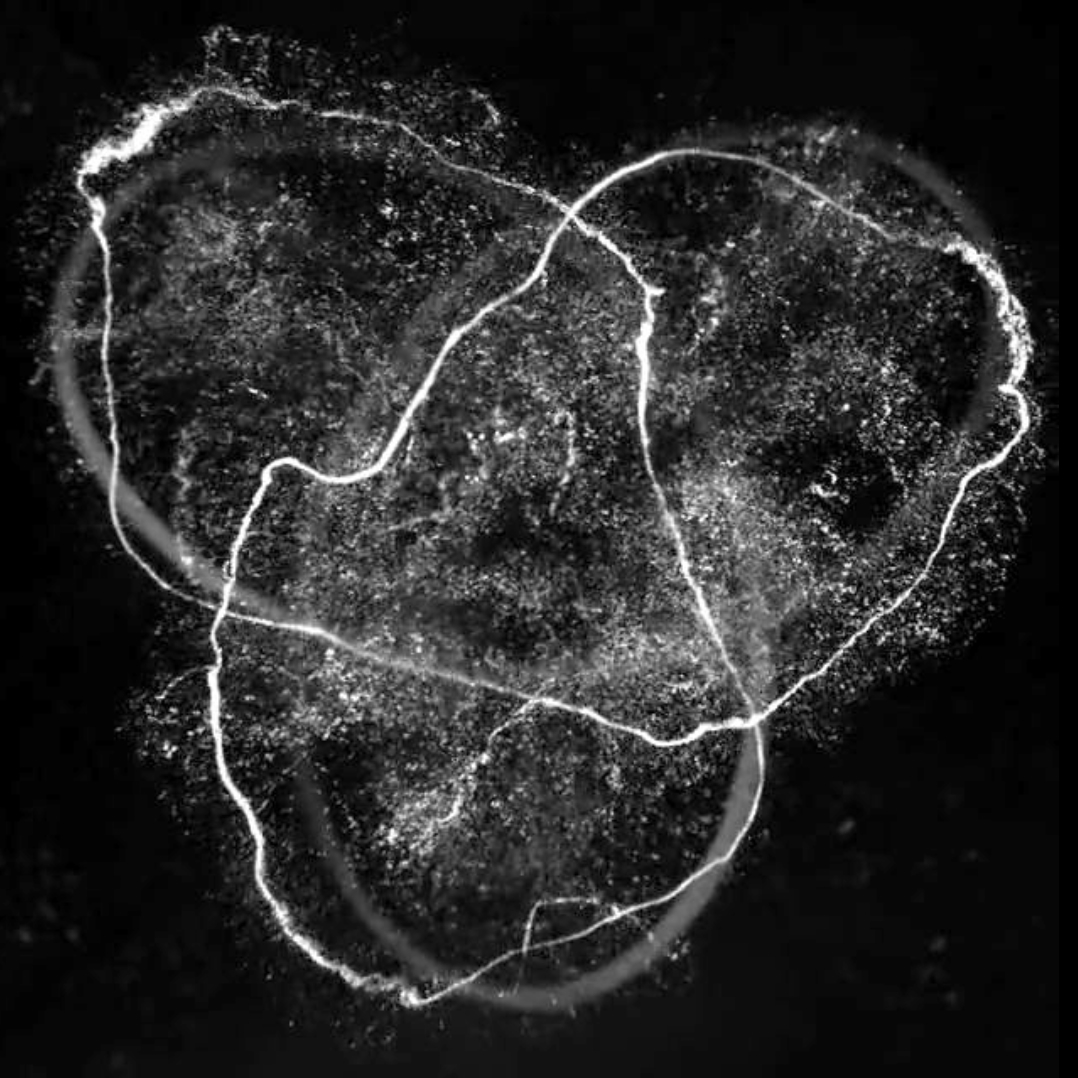
\includegraphics[width=\linewidth]{Pictures/knottedwatervortex}}
		\end{figure}
			\vspace{-2ex}
			\alert{Such fluid configurations are proved to exist both 
			\underline{theoretically} and \underline{experimentally}!}
	\end{column}
	\end{columns} 
\end{frame}
\note[itemize]{
	\item One of the  the main goal of our paper\cite{Miti2018} is to find an application of this construction in knot theory.
	\item The cornerstone of this idea is to recognize the ubiquitous role of the group of preserving diffeomorphisms. 
	The first step is to notice that conserved quantities can be associated to any fluid configurations (especially knotted ones).
 	\item The gist of the second proposition is that the topology of the support of the vorticity is conserved along the fluid evolution.
 	\item The image on the right represents a fluid configuration with knotted vorticity realized in the laboratory.
}
%------------------------------------------------------------------------------------------------

%-------------------------------------------------------------------------------------------------------------------------------------
\subsection{Basics of Knot theory}
%-------------------------------------------------------------------------------------------------------------------------------------
  \begin{frame}[fragile]{Basics of \emph{knots theory}}
		\begin{columns}
			\begin{column}[T]{.4\linewidth}
				\begin{figure}
					\caption{Reidmeister's move}
				\ifHandout
					\includestandalonewithpath[width=\textwidth,keepaspectratio]{./Pictures}{Figure_trefoil}
				\else
					\includestandalonewithpath[width=\textwidth,keepaspectratio]{./Pictures}{Animation_trefoil}
				\fi
				\end{figure}
			\end{column}
				\hfill
			\begin{column}[T]{.6\linewidth}
				\begin{enumerate}
					\item Knots = compact submanifolds of codimension 2 embedded in $\mathbb{R}^3$
						\begin{defblock}[n-link]
							%Disjoint union is written using \coprod, since it is in fact the coproduct in the category of sets.(\amalg)
							$\gamma: {\displaystyle\coprod_1^n S^1 } \to \mathbb{R}^3 $ embedding.				
						\end{defblock}
					\item studied \emph{modulo "ambient isotopies"}
						\begin{defblock}[Ambient isotopies]
							%Disjoint union is written using \coprod, since it is in fact the coproduct in the category of sets.(\amalg)
							$h : {\displaystyle\coprod_1^n S^1 }\times [0,1] \to \mathbb{R}^3 $ smooth homotopy
							s.t. $\hat{h}(t) : {\displaystyle\coprod_1^n S^1 } \to \mathbb{R}^3$ is an embedding $\forall t$	.				
						\end{defblock}	
					\item Holy grail of knot theory: classify all non equivalent (by ambient isotopies) n-links.
					\item \alert{These classes are invariant w.r.t. volume preserving diffeos.}
				\end{enumerate}
				%			
  	  \end{column}
    \end{columns}
	%
 \end{frame}
\note{
	\begin{itemize}
		\item It is possible to build a bridge between knot theory and multisymplectic geometry exploiting the tight connection between both of them with hydrodynamics.\\
		The cornerstone of this relationship is the ubiquitous role of the group of volume preserving diffeomorphisms.
		\item Knot  theory is not simply an instance of studying the topology of loops but the ambient space takes a significant role"
		\item Studying smooth knots is equivalent to study \href{http://mathworld.wolfram.com/PolygonalKnot.html}{tamed polygonal knots}.
		\item choosing a smooth parametrization is tantamount to fix an orientation of the knot.
	\end{itemize}
}
%-------------------------------------------------------------------------------------------------------------------------------------

%-------------------------------------------------------------------------------------------------------------------------------------
\subsection{Intermezzo: Poincare duals}
%------------------------------------------------------------------------------------------------

%------------------------------------------------------------------------------------------------
\begin{frame}{Recall: De Rham currents}
	On smooth manifolds is possible to mimick the basic definition of distribution using differential forms:
		\begin{defblock}[De Rham k-Currents]
			\begin{displaymath}
				\mathcal{D}_k(M)
				:= 
			\biggr\{\eta: \Omega^k_c(M)\rightarrow \mathbb{R} \; \left\vert \; \text{\stackanchor{(seq.) continuous}{linear functionals}} \right\} 
				\cong
				\left(\Omega^k_c (M) \right)^\ast
			\end{displaymath}
		\end{defblock}
		%
		\vspace{-2.5ex}
		%
  	\onslide<2->{
  	\begin{columns}
		\begin{column}[t]{.5\linewidth}	
			\begin{defblock}[Annihilation set of $T \in \mathcal{D}$]
				Open subset $A \subset M$ s.t. \\ 
				$\langle T, \phi \rangle = 0 \quad \forall \phi 	
				\text{ s.t. } \text{supp}(\phi) \subset A$
			\end{defblock}
		\end{column}
		\begin{column}[t]{.5\linewidth}			
			\begin{defblock}[Support of $T \in \mathcal{D}$]
				$\text{supp}(T)$ = complement of the union of all open annihilation sets of $\eta$
			\end{defblock}
		\end{column}
  	\end{columns}
  	}		
%
  	\onslide<3->{
	  	We have the analogue of \emph{regular distributions}
			\begin{alignat*}{2}
			  D:\Omega^k(M) & \longrightarrow & \mathcal{D}^{n-k}(M) & \\
			  \eta & \longmapsto & D_\eta & \quad:\quad 
			  \langle D_\eta, \text{\textvisiblespace} \rangle = 
			  \int_M \blank \wedge \eta \\
			  \text{d}\sigma& \longmapsto & D_{\text{d}\sigma} & \quad:\quad 
			  \langle D_{\text{d}\sigma}, \blank \rangle = 
			  (-)^{k} \int_M   \text{d}\blank \wedge\sigma
			\end{alignat*}	  	
  	}				
		%
		\vspace{-2.5ex}
		%
  	\onslide<4->{
		\begin{defblock}[De Rham boundary operator]
			\begin{displaymath}
				\partial : \mathcal{D}_k(M) \rightarrow \mathcal{D}_{k-1}(M) \qquad \text{s.t.} \quad
				\langle \partial T, \blank \rangle = (-)^{k} \langle T, \text{d}\blank \rangle
			\end{displaymath}
		\end{defblock}
  	}							
\end{frame}
\note[itemize]{
	\item this is the analogue of the theory of distribution on $\mathbb{R}^n$
	\item Continuity in the sense of distributions means \emph{sequentially continuous} i.e
		If a sequence $\omega_{k}$ of smooth forms, all supported in the same compact set, is such that all derivatives of all their coefficients tend uniformly to 0 when 
		$k$ tends to infinity, then $T(\omega_{k})$ tends to 0.
	\item $\Omega^k_c(M)$ stands for compact supported k-forms.
	\item Recall the definition of \emph{support} of a differential form
		$$
			\text{supp}(\omega) := \overline{\lbrace p \in M \; \vert \: \omega_p = 0 \rbrace}
		$$
	\item from the definition of regular distribution we obtain the definition of boundary operator.	
	\item De Rham distributions build up a chain complex which is dual (modulo a sign) to the de Rham co-chain complex.
}
%------------------------------------------------------------------------------------------------



%------------------------------------------------------------------------------------------------
\begin{frame}{Recall:Poincaré duals}
	Given a compact, oriented embedded k-dim submanifold $\Sigma$ of $M$ (n-dim)
	\begin{displaymath}
		\left( i : 	\Sigma \hookrightarrow M \right) \in \text{Emb}_c(k)
	\end{displaymath}		
	you can associate a compactly supported \emph{DeRham current} $D_\Sigma$ defined as
	\begin{displaymath}
		\langle D_\Sigma, \omega\rangle = \int_\Sigma i^\ast (\omega) \qquad 
		\forall \omega \in \Omega^k
	\end{displaymath}
		%
		\vspace{-2.5ex}
		%
	\onslide<2->{
  	\begin{columns}
		\begin{column}[c]{.5\linewidth}	
			\begin{claimblock}
				$\partial D_\Sigma = (-)^{k-1} D_{\partial \Sigma}$ 
			\end{claimblock}
		\end{column}
		\begin{column}[c]{.5\linewidth}			
			\begin{claimblock}
				$ D_{\Sigma_1} \wedge D_{\Sigma_2} = D_{\Sigma_1 \cap \Sigma_2}$
			\end{claimblock}
		\end{column}
  	\end{columns}
  }		
	%
	\onslide<3->{
		\begin{table}[]
		\begin{tabular}{lll}
			Analogue of the Dirac delta function localized on $\Sigma$ & $\Rightarrow$ & 
			\alert{\danger non regular \danger}
		\end{tabular}
		\end{table}

		We're interested in a \emph{regular approximation} (regularization)
		\begin{defblock}[a (smooth) Poincaré dual of $\Sigma$]
		 $\eta_\Sigma \in \Omega^k$ supported on a tubular neighbourhood $T$ of $\Sigma$ s.t.
		 \begin{displaymath}
				\langle D_{\eta_\Sigma},\omega\rangle \equiv \int_M \omega \wedge \eta_\Sigma =
				\int_T i^\ast \omega \sim 
				\langle D_{\Sigma},\omega\rangle 
		 \end{displaymath}
		\end{defblock}		
		  	\centering \alert{\danger \; ( Not unique! ) \; \danger}

  }		
\end{frame}
\note[itemize]{
	\footnotesize
	\item $\forall$ compact submanifold (dim=k) of $M$ (dim= n) one can associates a unique
	 de Rham current. 
	They can be understood as \emph{generalized} differential $(n-k)$-forms concentrated on $\Sigma$.
	This is the analogue of the Dirac delta function localized on $\Sigma$.
	\item Usual definition of Poincar\'e dual (in algebraic topology) is different:
	\\
		%\begin{defblock}[Poincaré dual of $\Sigma$]
			Unique $[\eta_\Sigma ] \in H^{n-k}_c(M)$ s.t.
			\begin{displaymath}
				\int_\Sigma i^\ast \omega = \int_M \omega \wedge \eta_\Sigma \qquad \forall [\omega] \in H^k(M)
			\end{displaymath}
		%\end{defblock}
		More conceptually, Poincaré duals can be seen as \emph{Thom Classes}.
	
	\item Proof of claim 1 is direct:
		\begin{displaymath}
			(-)^{k-1} \langle \partial D_\Sigma , \omega \rangle = 
			\langle D_\Sigma, d\omega\rangle =
			\int_\Sigma i^\ast d \omega = 
			 \int_\Sigma d i^\ast \omega = 
			 \int_{\partial \Sigma} i^\ast \omega =
			\langle D_{\partial \Sigma}, \omega \rangle
		\end{displaymath}
	\item Claim 2 is better understood with smooth Poincarè duals:
		\begin{displaymath}
			\text{supp}(\eta_1 \wedge \eta_2) \subset
			\text{supp}(\eta_1) \cap \text{supp}(\eta_2) \subset
			T_{\Sigma_1 \cap \Sigma_2} \quad\Rightarrow\quad
			\eta_1 \wedge \eta_2 = \eta_{\Sigma_1 \cap \Sigma_2}	
		\end{displaymath}				
		An example: 
		Take as $\Sigma_1$ the $z$-line in $\mathbb{R}^3$, $\eta_1 = \delta_{\{x=y=0\}}	dx \wedge dy$, and as $\Sigma_2$ the $xy$-plane, $\eta_2= \delta_{\{z=0\}} dz$.
		You get $\eta_1 \wedge \eta_2 = \delta_{\{x=y=z=0\}} dx \wedge dy \wedge dz = \eta_{\Sigma_1 \cap \Sigma_2}$
}
%------------------------------------------------------------------------------------------------




%-------------------------------------------------------------------------------------------------------------------------------------
\subsection{Invariant quantities related to knotted configurations}
%------------------------------------------------------------------------------------------------
\begin{frame}{Hamiltonian forms related to a n-link}

		
  	\onslide<1->{
  	\begin{columns}
		\begin{column}[c]{.7\linewidth}	
				Let $ L = \cup_{i=1}^n L_i$ be an oriented link in ${\mathbb R}^3$ 
				\\(components $L_i$, $i=1,\dots,n$ required to be  {\it trivial} knots)	
		\end{column}
		\begin{column}[c]{.25\linewidth}	
			\centering{
			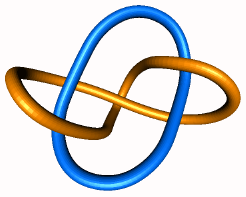
\includegraphics[width=0.75\linewidth]{Pictures/Whiteheadlink}
			}
		\end{column}
  	\end{columns}
  	}
		%
  	\onslide<2->{
  	\begin{columns}
		\begin{column}[t]{.5\linewidth}	
			\begin{defblock}[Vorticity 2-form]
				$$
				\omega_{L} := \sum_{i=1}^n \omega_{L_i}, \qquad d\omega_L = 0
				$$
				($\omega_{ L_i}$ = Poincar\'e dual associated to $L_i$)
			\end{defblock}
		\end{column}
		\begin{column}[t]{.5\linewidth}	
			\begin{defblock}[Velocity 1-form]
				$$
 					v_{ L} = \sum_{i=1}^n v_{L_i}, \qquad \qquad  dv_{L} = \omega_{ L}
				$$
				($v_{L_i} := \omega_{{\mathfrak a}_i}$ = Poincar\'e dual  of a disc ${\mathfrak a}_i$ 
				bounded by 	$L_i$ \footnotesize{(Seifert surface)}) 
			\end{defblock}						
		\end{column}
  	\end{columns}
  	}
  	%
  	\begin{columns}
		\begin{column}[t]{.3\linewidth}	
  		\onslide<2->{
  			\center
  			\vspace{-4ex}
				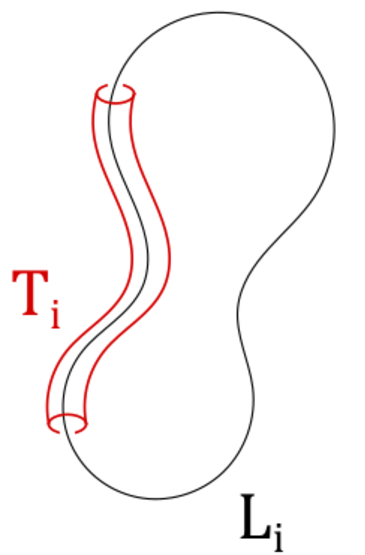
\includegraphics[width=0.6\linewidth]{Pictures/tubes}
	  	}			
		\end{column}
		\begin{column}[t]{.7\linewidth}	
  	\onslide<3->{
			\begin{propblock}[$v_{L}$ is a {\it Hamiltonian 1-form}]
				For each component $L_i$, the Hamiltonian vector field $\xi_{L_i}$ of 
				$v_{L_i}$ is $-\alpha^{-1}(\omega_{L_i})$.
				\\
				Explicitly, one has 
				\begin{displaymath}
					dv_L + \sum_{i=1}^n\iota_{\xi_{L_i}} \nu = 0 				
				\end{displaymath}
			\end{propblock}  	
  	}				
		\end{column}
  	\end{columns}
\end{frame}
\note[itemize]{
	\item $\omega_{ L_i}$ denote the Poincar\'e (or Thom) dual (class) associated to $L_i$: they are 2-forms localized in a 
 cross-section of a  suitable tubular neighbourhood $T_i$ around $L_i$ - with total fibre integral equal to one, or, as currents, 2-forms which are $\delta$-like on $L_i$
 
	\item $v_{L_i} := \omega_{{\mathfrak a}_i}$ is the Poincar\'e dual (class) of a disc ${\mathfrak a}_i$ bounding
$L_i$ (a Seifert surface for the trivial knot $L_i$). Precisely:
$$
\partial {\mathfrak a}_i = L_i, \qquad \qquad dv_{L_i} = d\omega_{{\mathfrak a}_i} = \omega_{L_i} = \omega_{\partial {\mathfrak a}_i},
$$
	\item
		Velocity 1-forms $v_i$ correspond (upon approximation of the associated Euler equation) to the so-called LIA (Linear Induction Approximation) or  {\it binormal evolution}
		of the ``vortex ring" $L_i$ (``orthogonal" to the discs ${\mathfrak a}_i$.
		
	\item Everything is up to choices of tubular neighbourhoods, Seifert surface and specific Poincar\'e dual.


}
%------------------------------------------------------------------------------------------------


%------------------------------------------------------------------------------------------------
\begin{frame}{Relation with Gauss linking number}
		%
		\vspace{-2.5ex}
		%
  	\begin{columns}
		\begin{column}[t]{.5\linewidth}	
			\begin{defblock}[Chern-Simons 3-form]
				$$
					CS({L}) :=  v_{L} \wedge  \omega_{ L} 
				$$
			\end{defblock}
		\end{column}
		\begin{column}[t]{.5\linewidth}	
			\begin{defblock}[Helicity]
				$$
 					{\mathcal H}(L) = \int_{\mathbb{R}^3} CS({L})
				$$
			\end{defblock}						
		\end{column}
  	\end{columns}
	\pause
	\begin{propblock}[
		Choosing a parametrization $\mathbf{r}_i$ (in standard coordinates) for each $L_i$ 
		\begin{displaymath}
			{\mathcal H}(L)  = 
			\sum_{i,j=1}^n
			\,\frac{1}{4\pi}
			\oint_{\gamma_i}\oint_{\gamma_j}
			\frac{\mathbf{r}_i - \mathbf{r}_j}{|\mathbf{r}_i - \mathbf{r}_j|^3}
			\cdot (d\mathbf{r}_i \times d\mathbf{r}_j) =
			\sum_{i,j=1}^n \ell(i,j)
		\end{displaymath}
			$\bullet$ $\ell(i,j) = \ell(j,i)$ : Gauss linking number of components $L_i$ and $L_j$ if $i\neq j$\\
			$\bullet$ $\ell(j,j)$ : {\it framing} of $L_j$\\ 
			\phantom{-------}\footnotesize{ (i.e. $\ell(L_j, L_j^{\prime})$ with $L_j^{\prime}$ being a section of the normal bundle of $L_j$.)}\normalsize

		]
	\pause
  	\begin{columns}
		\begin{column}[c]{.7\linewidth}	
		\underline{Sketch}: Cosider a Hopf Link
			\begin{displaymath}
				L(C,C') = \eta_C \wedge \eta_{\Sigma'} + \eta_{C'} \wedge \eta_\Sigma =
				\eta_{P'} + \eta_{P}
			\end{displaymath}
		\end{column}
		\begin{column}[c]{.25\linewidth}	
			\centering{
			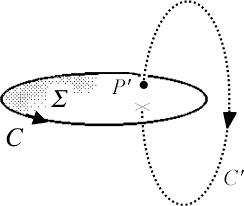
\includegraphics[width=0.75\linewidth]{Pictures/GaussLink}
			}
		\end{column}
  	\end{columns}
			Therefore $\int L(C,C') = \ell(C,C')$ is counting the times that a knot cross another Seifert surface with sign given by the orientation.
		\end{propblock}
		
\end{frame}
\note[itemize]{
	\item Our previous construction is heavily dependent on a lot of choices 
	but we end up with a quantity that only depends on the starting n-link.
	\item ${\mathcal H}(L)$ is invariant under ambient isotopies.\\
	However, non ambient isotopic links do not necessarily yield different linking numbers
	(it is not an universal invariant!).
  	\begin{columns}
		\begin{column}[c]{.5\linewidth}	
			\centering{
			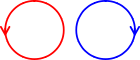
\includegraphics[width=0.5\linewidth]{Pictures/UnknotsGauss}
			}
		\end{column}
		\begin{column}[c]{.5\linewidth}	
			\centering{
			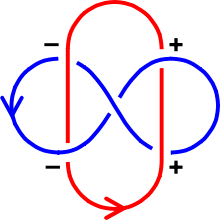
\includegraphics[width=0.35\linewidth]{Pictures/WhiteheadGauss}
			}
		\end{column}
  	\end{columns}	
	\item
		\begin{displaymath}
	\begin{split}
		\text{link}(\gamma_1,\gamma_2) &=\,\frac{1}{4\pi}
		\oint_{\gamma_1}\oint_{\gamma_2}
		\frac{\mathbf{r}_1 - \mathbf{r}_2}{|\mathbf{r}_1 - \mathbf{r}_2|^3}
		\cdot (d\mathbf{r}_1 \times d\mathbf{r}_2)\\[4pt]
		 &= \frac{1}{4\pi}\int_{S^1 \times S^1} \frac{\text{det}(\dot{\gamma_1}(s),
	 \dot{\gamma_2}(t),\gamma_1(s)-\gamma_2(t))}{|\gamma_1(s)-\gamma_2(t)|^3}\, ds \, dt
	\end{split}
	\end{displaymath}			
}
%------------------------------------------------------------------------------------------------

%-------------------------------------------------------------------------------------------------------------------------------------
\subsection{Higher order link invariants}
%------------------------------------------------------------------------------------------------

%------------------------------------------------------------------------------------------------
\begin{frame}{Cohomological interpretation of the linking number}
		\vspace{2ex}
  	\begin{columns}
		\begin{column}[c]{.75\linewidth}	
			$\bullet$ Choose a pair of linked knots (part of a more complex link).
			Define
			$$ \Xi_{1 2} := - v_{L_1} \wedge v_{L_2} \in \Omega^2(\mathbb{R}^3)$$
			you get:
			\begin{displaymath}
				\begin{split}
				d \Xi_{1 2} =& -\omega_1 \wedge v_2 + v_1 \wedge \omega_2 = CS({L_1\cup L_2}) - 
				\text{"\stackanchor{self}{linking}"}
				\\
				&\Rightarrow \int d \Xi_{1 2} = \ell(1,2)
				\end{split}
			\end{displaymath}		
		\end{column}
		\begin{column}[c]{.20\linewidth}	
			\centering{
			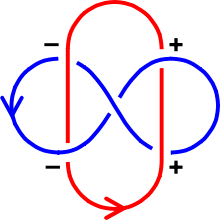
\includegraphics[width=\linewidth]{Pictures/WhiteheadGauss}
			}
		\end{column}
  	\end{columns}	
	\pause	
	\vspace{1ex}
	$\bullet$ While $\Xi_{1 2}$ is not uniquely defined,it determines an unique class in the \emph{cohomology of the link}
	(independent of the choices)
	\begin{displaymath}
		\langle L_1, L_2 	\rangle := 
		\left[\Xi_{1 2}\bigg\rvert_{S^3\setminus L} \right] \in H^2(S^3\setminus L)
	\end{displaymath}
	\pause
	\vspace{-2ex}
  	\begin{columns}
		\begin{column}[c]{.72\linewidth}	
			\begin{propblock}[$\ell(1,2)= 0 \Leftrightarrow \langle L_1, L_2 \rangle = 0$]
				\vspace{-4ex}
				\begin{displaymath}
				\begin{split}
					l(1,2)=0 \quad&\Leftrightarrow\quad d \Xi_{1 2} = 0 \in \Omega^2(\mathbb{R}^3)\\
					\text{"Poincar\'e lemma"}	
					\quad&\Rightarrow\quad \exists v_{1 2} \;:\; d v_{1 2} = \Xi_{ 1 2}	\\
					[ \Xi_{1 2} ] = 0 \in H^2(\mathbb{R}^3) \quad&\Rightarrow\quad
					\left[\Xi_{1 2}\bigg\rvert_{S^3\setminus L} \right] = 0 \in H^2(S^3\setminus L)
				\end{split}
				\end{displaymath}		
			\end{propblock}
		\end{column}
		\begin{column}[c]{.3\linewidth}	
	  	\begin{asideblock}[Cohomology groups of a n-Link]%Shades of...
  			\begin{table}[] % http://tablesgenerator.com/
					\begin{tabular}{l}
						$H^0 (S^3 \setminus L) \cong {\mathbb R}$ \\
						$H^1 (S^3 \setminus L) \cong {\mathbb R}^{n}$ \\
						$H^2 (S^3 \setminus L) \cong {\mathbb R}^{n-1}$ \\
						$H^3 (S^3 \setminus L) \cong 0$
					\end{tabular}
				\end{table}
	  	\end{asideblock}
		\end{column}
  	\end{columns}			



	

\end{frame}
\note[itemize]{
	\item The cohomology of a n-link is the de Rham cohomology of $S^3 \setminus L$, 
	where $S^3$ has to be understood as the compactification of the Euclidean space
	\item Being $\Xi_{1 2}$ closed follows from the fact that 
	$\text{supp}(d \Xi_{1 2}) \subseteq L$ \\
	Similarly, you get that all the velocity 1-forms $v_i$ are closed.
	The cohomology classes of these forms, one for each component of the link, 
	are precisely the generators of $H^1 (S^3 \setminus L)$.
	\item Why such a class is called a number? 
	The name follows from the simplest case of $n=2$.
	\item \underline{Upshot:} we can associate to any pair of knots in a link a  cohomology class.
}
%------------------------------------------------------------------------------------------------

%------------------------------------------------------------------------------------------------
\begin{frame}{Higher order linking numbers}
	\begin{itemize}
		\item[•] Take a link with 3 or more components
		\item[•] 	assume all ordinary mutual linking numbers vanish: $\langle L_i, L_j \rangle =0$
		\item[•] Out of the primitives obtained in the previous proposition you can manufacture another closed 2-form
	\end{itemize}
		\vspace{-2ex}
  	\begin{columns}
		\begin{column}[c]{.5\linewidth}	
			\begin{defblock}[Massey product]
				$\Xi_{1 2 3} = - v_1 \wedge v_{2 3} - v_{1 2} \wedge v_3 
				\in \Omega^2(\mathbb{R^3})$
			\end{defblock}
		\end{column}
		\begin{column}[c]{.5\linewidth}	
			\begin{defblock}[Third order linking number (class)]
				$\langle L_1, L_2, L_3 \rangle := 
				\left[\Xi_{1 2 3}\bigg\rvert_{S^3\setminus L} \right]
				\in H^2(S^3\setminus L)$
			\end{defblock}
		\end{column}
  	\end{columns}			
  	\pause
	The procedure can be iterated (obstructed by the non vanishing of a higher linking number) yielding a hierarchy of pairs
	\begin{displaymath}
		\Xi_I \in \Omega^2 \qquad v_I \in \Omega^1
	\end{displaymath}
	\center
	\footnotesize{(I = multi index constructed out of the set $\{1,\ldots,n\}$ of the $n$-link components)}\normalsize 

	\pause 	\center 	\textbf{-- Applications --}
  	\begin{columns}
		\begin{column}[c]{.45\linewidth}
			Distinguish different links with same (vanishing) Gauss linking number	
			\center
			\begin{tikzpicture}
			\node[inner sep=0pt] (A) at (0,0)
			    {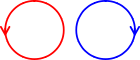
\includegraphics[width=.4\textwidth]{Pictures/UnknotsGauss}};
			\node[inner sep=0pt] (B) at (3,0)
			    {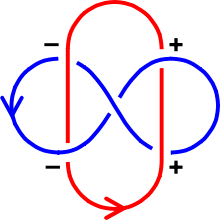
\includegraphics[width=.4\textwidth]{Pictures/WhiteheadGauss}};
			\draw[draw=none] (A) -- (B)
			    node[midway,fill=white] {$ \not\sim $};
			\end{tikzpicture}
		\end{column}
		\hspace{2ex}
		\begin{column}[c]{.45\linewidth}	
			Ascertain \emph{Brunnian character}
			\centering{
			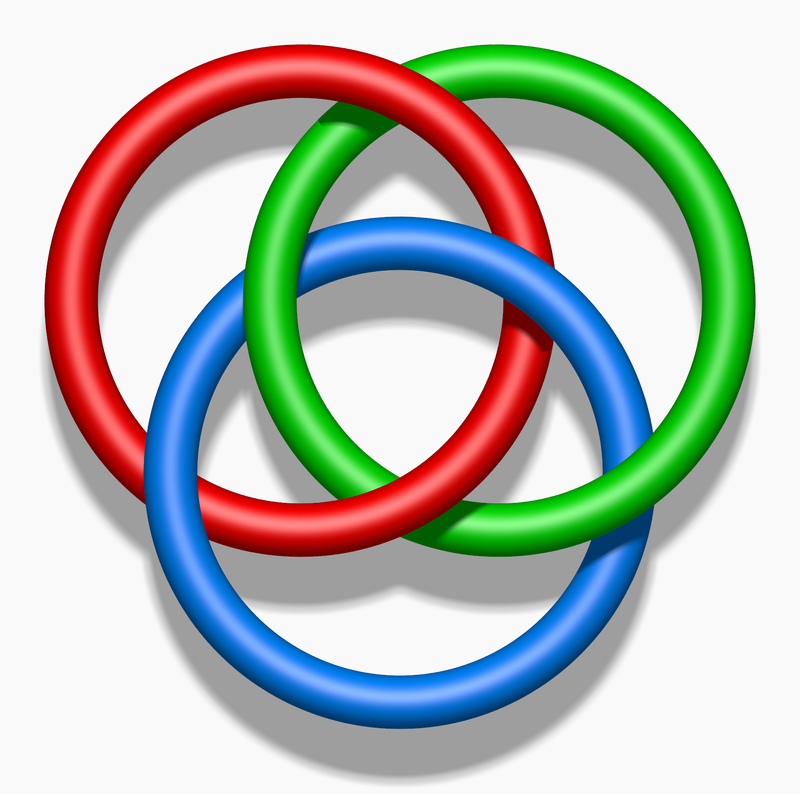
\includegraphics[width=0.5\linewidth]{Pictures/BorromeanLink}
			}
		\end{column}
  	\end{columns}			



\end{frame}
\note[itemize]{
	\item $\Xi_I$ and $v_I$ can be again interpreted via Poincar\'e duality as the smooth Poincar\'e dual of an auxiliary trivial knot and of a corresponding Seifert surface respectively.
	\item Below, two possible application of this machinery are mentioned .
	\item This procedure can be used as a tool to distinguish knots with vanishing linking number. (Figure: two unknots versus a Whithead Link. The latter involve forth order linking numbers computing admitting indices repetition).
	\item Ascertain the Brunnian character of a $n$-link. A link is \emph{Brunnian} 
		or \emph{almost trivial} when it becomes trivial upon removing any component. 
		(Figure: Borromean link).
}
%------------------------------------------------------------------------------------------------

%------------------------------------------------------------------------------------------------
\begin{frame}{Massey products as Conserved quantities}
	%
	\begin{propblock}[
		\quad(1) $\Xi_I$ exact $\Rightarrow$ $v_I$ are hamiltonian (w.r.t volume form) \\
		\phantom{-------------}(2) Massey 2-forms $\Xi_I$ are globally conserved
		]
		\vspace{-4ex}
		\begin{displaymath}
		\begin{split}
			(1)&\quad d v_{I} = \Xi_{I} = \iota_{\xi_{I}} \text{Vol}_{\mathbb{R}^3} \qquad 
			\text{defining}\quad \xi_{I} = \alpha^{-1}(\Xi_{I})
			\qquad \Rightarrow \text{$v_{123}$ Hamiltonian}
			\\
			(2)&\quad \Xi_I \text{ closed} \quad \Rightarrow \quad \mathcal{L}_\xi \Xi_I = d \iota_xi \Xi_I \in B^2
		\end{split}
		\end{displaymath}

	\end{propblock}	
	By construction: the momenta associated to the divergence-free field $\xi_{I}$
	 correspond to $v_I$
		\begin{displaymath}
			v_I = f_1(\xi_I)
		\end{displaymath}
	\pause \vfill
	\begin{propblock}[
		The 1-forms $v_I$ are {\rm first integrals in involution} with respect to the flow generated by the 
		Hamiltonian vector field $\xi_{ L}$, i.e.
		\begin{itemize}
			\item ${\mathcal L}_{\xi_{ L}} v_I = 0$ ($v_I$'s are  {\rm strictly conserved})
			\item $\{v_I, v_J \} = 0$ (for multiindices $I$ and $J$)
		\end{itemize}
	]


	See Thm 6.2 \href{https://arxiv.org/abs/1805.01696}{arXiv: 1805.01696}
	\end{propblock}	
	
	

\end{frame}
\note[itemize]{
	\item $\xi_{123} = \alpha^{-1}(\Xi_{123})$, constructed resorting on the Hodge machinery of $\mathbb{R}^3$ can be regarded as the vorticity field concentrated on a auxiliary knot.
	\item {\bf Proof. Thm 6.2} Using Cartan's formula, we get
		$$
			{\mathcal L}_{\xi_{ L}} v_I = d \iota_{\xi_{ L}} v_I + \iota_{\xi_{ L}} d v_I = 
			d \iota_{\xi_{ L}} v_I  -  \iota_{\xi_{ L}} \iota_{\xi_{ I}} \nu,
		$$
		but the second summand vanishes in view of the general expression
		$$
			\{v_\xi, v_\eta \}(\cdot) = \nu (\xi, \eta, \cdot)
		$$
		and of the peculiar structure of the vector fields involved (they either partially coincide or have disjoint supports). 
		By the same argument, one gets $\iota_{\xi_{ L}} v_I = 0$. From that the the {\it strict} conservation of the $v_I$'s is immediate.\par
	\item  Poincar\'e dual interpretation $\Rightarrow$ $\iota_{\xi_{ L}} v_L = 0$
		$\Rightarrow$ ${\mathcal L}_{\xi_{ L}} v_L = 0 $
		\\
		(this is {\it not} to be expected a priori in multisymplectic geometry)


}
%------------------------------------------------------------------------------------------------


\end{document}
